\documentclass[14pt, a4paper]{extarticle}
\usepackage{GOST}
\usepackage{array}
\usepackage{verbatim}
\usepackage[detect-all]{siunitx}
\usepackage{amsmath}
\usepackage{amssymb}
\usepackage[utf8]{inputenc}
\usepackage{hyperref}

\usepackage{ifthen}


\usepackage{tempora}



\makeatletter
\renewcommand\@biblabel[1]{#1.}
\makeatother

% Для листинга кода:
\usepackage{listings}
\lstset{ %
	language=c++,                 % выбор языка для подсветки (здесь это С)
	basicstyle=\small\sffamily, % размер и начертание шрифта для подсветки кода
	numbers=left,               % где поставить нумерацию строк (слева\справа)
	numberstyle=\tiny,           % размер шрифта для номеров строк
	stepnumber=1,                   % размер шага между двумя номерами строк
	numbersep=5pt,                % как далеко отстоят номера строк от подсвечиваемого кода
	showspaces=false,            % показывать или нет пробелы специальными отступами
	showstringspaces=false,      % показывать или нет пробелы в строках
	showtabs=false,             % показывать или нет табуляцию в строках
	frame=single,              % рисовать рамку вокруг кода
	tabsize=2,                 % размер табуляции по умолчанию равен 2 пробелам
	captionpos=t,              % позиция заголовка вверху [t] или внизу [b] 
	breaklines=true,           % автоматически переносить строки (да\нет)
	breakatwhitespace=false, % переносить строки только если есть пробел
	escapeinside={\#*}{*)}   % если нужно добавить комментарии в коде
}


%для графиков
\usepackage{pgfplots}
\usepackage{filecontents}
\usetikzlibrary{datavisualization}
\usetikzlibrary{datavisualization.formats.functions}
\begin{filecontents}{pr.dat}
	0 0
	100 154
	200 308
	300 460
	400 615
	500 768
	600 922
	700 1075
	800 1232
	900 1386
	1000 1540
\end{filecontents}

\begin{filecontents}{prOGL.dat}
	0 0
	100 0
	200 0
	300 0
	400 0
	500 0
	600 0
	700 0
	800 0
	900 0
	1000 1
\end{filecontents}

\begin{document}
	
	\begin{table}[ht]
		\centering
		\begin{tabular}{|c|p{400pt}|} 
			\hline
			\begin{tabular}[c]{@{}c@{}} 
\includegraphics[scale=1]{source/baum.jpg} \\\end{tabular} &
			\footnotesize\begin{tabular}[c]{@{}c@{}}\textbf{Министерство~науки~и~высшего~образования~Российской~Федерации}\\\textbf{Федеральное~государственное~бюджетное~образовательное~учреждение}\\\textbf{~высшего~образования}\\\textbf{«Московский~государственный~технический~университет}\\\textbf{имени~Н.Э.~Баумана}\\\textbf{(национальный~исследовательский~университет)»}\\\textbf{(МГТУ~им.~Н.Э.~Баумана)}\\\end{tabular}  \\
			\hline
		\end{tabular}
	\end{table}
	\noindent\rule{\textwidth}{4pt}
	\noindent\rule[14pt]{\textwidth}{1pt}
	\hfill 
	\noindent
	\makebox{ФАКУЛЬТЕТ~}%
	\makebox[\textwidth][l]{\underline{~«Информатика и системы управления»~~~~~~~~~~~~~~~~~~~~~~~~~~~~~~~~~}}%
	\\
	\noindent
	\makebox{КАФЕДРА~}%
	\makebox[\textwidth][l]{\underline{~«Программное обеспечение ЭВМ и информационные технологии»~}}%
	\\
	
	\begin{center}
		\vspace{1.5cm}
		{\bf\huge Расчётно-пояснительная записка\par}
		{\bf\Large к курсовому проекту\par}
		\vspace{0.7cm}
	\end{center}
	
	
	\noindent
	\makebox{\large{\bf Название:}~~~}
	\makebox[\textwidth][l]{\large\underline{Создание трёхмерной модели Земли~~~~~~~~~~~~~}}\\
	\makebox[\textwidth][c]{\large\underline{~~~~с визуализацией полётов самолетов~~~~~~~~~~~~~}}
	
	\noindent
	\makebox{\large{\bf Дисциплина:}~~~}
	\makebox[\textwidth][l]{\large\underline{~Компьютерная графика~~~~~~~~~~~~~~~~~~~~~~~~~~}}\\
	
	\vspace{1.5cm}
	\noindent
	\begin{tabular}{l c c c c c}
		Студент      & ~ИУ7-55Б~               & \hspace{2.5cm} & \hspace{2cm}                 & &  Д.В. 
		Сусликов \\\cline{2-2}\cline{4-4} \cline{6-6} 
		\hspace{3cm} & {\footnotesize(Группа)} &                & {\footnotesize(Подпись, дата)} & & {\footnotesize(И.О. Фамилия)}
	\end{tabular}
	
	\noindent
	\begin{tabular}{l c c c c}
		Преподователь & \hspace{5cm}   & \hspace{2cm}                 & & ~О.В. Кузнецова~\\\cline{3-3} \cline{5-5} 
		\hspace{3cm}  &                & {\footnotesize(Подпись, дата)} & & {\footnotesize(И.О. Фамилия)}
	\end{tabular}
	
	\vspace{0.6cm}
	\begin{center}	
		\vfill
		\large \textit {Москва, 2020}
	\end{center}
	
	\thispagestyle {empty}
	\pagebreak	
	
	% СОДЕРЖАНИЕ 
	\clearpage
	\tableofcontents
	
	
	% ВВЕДЕНИЕ
	\clearpage
	\section*{Введение}
	\addcontentsline{toc}{section}{Введение}
	Область применения компьютерной графики не ограничивается одними
	художественными эффектами. Во всех отраслях науки, техники, медицины,
	в коммерческой и управленческой деятельности используются построенные
	с помощью компьютера схемы, графики, диаграммы, предназначенные для
	наглядного отображения разнообразной информации.\par
	
	В наше время всё труднее и труднее становится следить за передвижениями людей по всему земному шару. Многие передвигаются на наземном, на водном, а так же на воздушном транспорте. Такие передвижения очень часто чреваты последствиями, что мы наблюдали в 2020 году. Распространение вируса осуществлялось преимущественно благодаря заболевшим, что путешествовали на самолётах. Следовательно, требуется модель для просмотра за передвижениями людей из одного города в другой. Поэтому задача создания модели Земли с визуализацией полётов самолетов актуальна сегодня, как никогда.\par
	
	Цель данной работы - разработать программное обеспечение для визуализации полётов самолетов над Землей.\par
	Для достижения поставленной цели необходимо решить следующие задачи:
	\begin{itemize}
		\item[1)] проанализировать существующие программные решения;
		\item[2)] разработать математическую модель и алгоритм для формирования модели Земли
		 и для построения траекторий полетов самолетов;
		 \item[3)] разработать программное обеспечение для визуализацией полётов самолетов на трехмерной модели Земли.
	\end{itemize}
	
	\clearpage
	\section{Аналитический раздел}
	В данном разделе расписано, что из себя представляет планета Земля, какие системы координат используются для её описания. Написано, что такое траектория. Так же непосредственно представлена сама задача.\par
	
	\subsection{Земля}
	Среди планет земной группы Солнечной системы, в которую входят Меркурий, Венера и Марс, Земля самая крупная. Планета третья по удаленности от Солнца, она является пятой по диаметру массе и плотности.\par
	Возраст нашей планеты сравнивают с возрастом всей Солнечной системы и насчитывает примерно 4,5 млрд лет. Существует гипотеза, что Земля образовалась из газа и пыли, которые остались от формирования солнца.\par
	Древнейшие горные породы, которые были изучены, образовывались примерно
	100 — 200 миллионов лет. А условия, благоприятные для возникновения жизни на планете, возникли только 3,5 млрд лет назад появились. Мы же, как современный тип человека, сформировались только 40 000 лет назад.\par
	
	Земля, и мы вместе с ней, вращается вокруг Солнца по круговой орбите, радиус которой составляет 150 млн км. Период, за который обращается по орбите Земля, происходит со скоростью 29,8 км/с и длится 365 суток. Приблизительное расстояние до Солнца составляет 149 543 000 километра.\par
	
	Земля вращается также вокруг своей воображаемой оси (с запада на восток). Полный оборот совершается примерно за 23 часа 56 минут. Ось вращения наклонена на
	66,5 градусов по отношению к плоскости орбиты, и в результате такого движения происходит смена дня и ночи. А так как земля одновременно ведет вращение вокруг Солнца, то приближаясь, то удаляясь от него — происходит смена времен года.\par
	
	
	Если рассматривать Землю со стороны геодезии и географии, то это планета имеет геоидную форму с радиусом 6378137 метров по экватору и 6356752 метра по полярному кругу. Планета поделена широтами и долготами(меридианами).\par
	Широта делится на южную и северную и изменяется от 0 до 90 градусов, разделяя Землю горизонтальные доли.\par
	Долгота делится на восточную и западную и изменяется от 0 до 180 градусов, разделяя Землю на вертикальные доли.

	\subsection{Полеты на самолетах}
	Никто не станет спорить с тем, что воздушный транспорт в современном мире наиболее востребованная техника.Количество регулярных пассажироперевозок до последнего времени росло постоянно, ежегодно наблюдалась тенденция к увеличению на 5-7\%. Ожидается, что до 2025 года каждый год пассажиропоток будет увеличиваться на 4-6\%.	
	Полеты на самолетах в современном мире, как и раньше, имеет огромное значение для человечества. Этот вид транспорта наделен множеством преимуществ. Характеризуется быстротой передвижения, возможностью оказаться в нужном месте за минимальный временной промежуток. При этом гарантируется комфорт в пути, разнообразный сервис. Именно поэтому авиатехника пользуется повышенным спросом. Например, на пассажироперевозки сегодня приходится 82\%, грузы – 14,7\%, почтовые отправления – 3,3\%. Рассмотрим, чаще всего и куда летают граждане разных стран мира.
	
	
	
	\subsection{Траектория}
	Траектория (от позднелатинского trajectories – относящийся к перемещению) – это линия, по которой движется тело (материальная точка). Траектория движения может быть прямой (тело перемещается в одном направлении) и криволинейной, то есть механическое движение может быть прямолинейным и криволинейным.\par
	
	Траектория прямолинейного движения в данной системе координат – это прямая линия. Например, можно считать, что траектория движения автомобиля по ровной дороге без поворотов является прямолинейной.\par
	
	Криволинейное движение – это движение тел по окружности, эллипсу, параболе или гиперболе. Пример криволинейного движения – движение точки на колесе движущегося автомобиля или движение автомобиля в повороте.\par
	
	Движение может быть сложным. Например, траектория движения тела в начале пути может быть прямолинейной, затем криволинейной. Например, автомобиль в начале пути движется по прямой дороге, а затем дорога начинает «петлять» и автомобиль начинает криволинейное движение.\par
	
	
		
	\subsection{Геодезическая система координат}
	
	Изначально все координаты объектов на Земле представлены в геодезическом виде, т.е. тремя координатами:
	широтой, долготой, высотой.\par 
	Геодезическая система координат — это система координат, используемая для определения местоположения объектов на Земле.\par
	
	Геодезические координаты используются в геодезии и навигации, в топографической съемке и картографии, а также спутниковыми навигационными системами для определения местоположения объектов на Земле в реальном времени.\par
			
	\subsection{Прямоугольная система координат}
	Прямоугольная система координат — прямолинейная система координат с взаимно перпендикулярными осями на плоскости или в пространстве. Наиболее простая и поэтому часто используемая система координат. Очень легко и прямо обобщается для пространств любой размерности, что также способствует её широкому применению.
	
	Для изображения объектов на экране используются прямоугольные координаты: x, y, z.
	
	\subsection{Преобразование координат}
	Для преобразования координат из реальных - геодезических в классическую - прямоугольную нужно знать:
	\begin{itemize}
		\item[1)] что из себя представляет геодезическая система координат;
		\item[2)] что из себя представляет прямоугольная система координат;
		\item[3)] каким образом осуществляется перевод из одной системы координат в другую.
	\end{itemize}

	\subsection{Афинные преобразования}
	Растяжения и сжатия, в определенном смысле, равномерные.	
	Эта равномерность означает, что все кусочки плоскости будут растягиваться (сжиматься) одинаково.
	Кроме того, когда мы растягиваем (сжимаем) квадрат, его стороны — отрезки остаются отрезками.	
	Такие равномерные растяжения (сжатия) называются аффинными преобразованиями.\par	
	Преобразование плоскости называется аффинным, если оно взаимно однозначно и образом любой прямой является прямая. Преобразование называется взаимно однозначным, если оно разные точки переводит в разные, и в каждую точку переходит какая-то точка.\par
	Частным случаем аффинных преобразований являются просто движения (без какого-либо сжатия или растяжения). Движения — это такие преобразования, которые сохраняют расстояние между любыми двумя точками неизменным, а именно параллельные переносы, повороты, различные симметрии и их комбинации.\par	
	Другой важный случай аффинных преобразований — это растяжения и сжатия относительно прямой.\par
	Есть еще важный класс аффинных преобразований — это сжатия и растяжения относительно точки. Они называются преобразованиями подобия или гомотетиями.
	
	Афинные пребразования обладают следующими свойствами:
	\begin{itemize}
		\item[1)] сохраняют линейные отношения между векторами;
		\item[2)] сохраняют отношения коллинеарных отрезков, 
		в частности, середины отрезков переходят в середины отрезков,
		а медианы треугольников, соответственно, в медианы образов этих треугольников;
		\item[3)] при аффинных преобразованиях отрезки
		переходят в отрезки, треугольники – в треугольники, тетраэдры – в тетраэдры;
		\item[4)] композиция аффинных преобразований плоскости
		является аффинным преобразованием плоскости.
	\end{itemize}
	
	\subsection{Постановка задачи}
	Разработать программное обеспечение для визуализации полётов самолетов над Землей. Изображение должно представлять собой трехмерную модель Земли, которую можно вращать и масштабировать. Реализовать отображение траекторий полётов самолетов и сами их передвигающиеся модели. Предоставить возможность отображения определённых траекторий из списка траекторий передвижений самолетов. Также реализовать возможность ускорить передвижение самолетов при помощи слайдера увеличения хода времени. Окно программы должно иметь фиксированный размер.
	
	\subsection*{Вывод}
	\addcontentsline{toc}{subsection}{Вывод}
	Таким образом, в данном разделе было разобрано, что из себя представляет планета Земля, какие системы координат используются для её описания, что такое траектория. Описана сама задача.
	
	\clearpage
	\section{Конструкторский раздел}
	В данном разделе будут рассмотрены требования к программе и алгоритмы решения поставленной задачи.
	
	\subsection{Требования к программе}
	Программа должна предоставлять следующие возможности:
	\begin{itemize}
		\item[1)] демонстрировать трехмерную модель Земли;
		\item[2)] поворот модели в любом направлении;
		\item[3)] масштабирование модели;
		\item[4)] предоставлять список доступных для выбора траекторий;
		\item[5)] отображать траекторию полетов;
		\item[6)] отображать передвижение самолетов по данной траектории.
	\end{itemize}
	
	\subsection{Общий алгоритм решения поставленной задачи}
	Алгоритм работы программы:
	\begin{itemize}
		\item[1)] демонстрировать трехмерную модель Земли;
		\item[2)] поворот модели в любом направлении;
		\item[3)] масштабирование модели;
		\item[4)] предоставлять список доступных для выбора траекторий;
		\item[5)] отображать траекторию полетов;
		\item[6)] отображать передвижение самолетов по данной траектории.
	\end{itemize}
	
	
	\subsection{Перевод из геодезической системы координат в прямоугольную}
	В геодезической системе координат положение точки определяется высотой Н, широтой В и долготой L. Такая эллипсоидальная система применяется при обработке наземных геодезических измерений. В космической геодезии при создании спутниковых геодезических сетей, которые являются пространственными и физически не связаны с какой-либо отсчет- ной поверхностью, более удобна система пространственных прямоугольных координат X, Y, X.\par
	Прямоугольные координаты точек в пространстве можно вычислить по известным геодезическим координатам этих точек (широта B, долгота L, высота H) по формулам:
	\begin{equation}
		X = (N(B) + H) cos(B) cos(L)
	\end{equation}
	
	\begin{equation}
		Y = (N(B) + H) cos(B) cos(L)
	\end{equation}

	\begin{equation}
		Z = (\frac{b^2}{a^2} N(B) + H) sin(B)
	\end{equation}

	где
	
	\begin{equation}
		ТN(B) = \frac{a^2}{\sqrt{a^2 cos^2((B) + b^2 sin^2(B))}} = \frac{a}{\sqrt{1 - e^2 sin^2(B)}},
	\end{equation}

	где a и b — экваториальный (большая полуось) и полярный радиусы (малая полуось), соответственно.
	$e^2 = \frac{a^2 - b^2}{a^2}$ — квадрат первого эксцентриситета эллипсоида.\par
	 N(B) радиус кривизны первого вертикала — расстояние по нормали к эллипсоиду от точки пересечения поверхности эллипсоида нормалью до оси oZ.
	
	\clearpage
	\subsection{Трехмерные преобразования}
	Рассмотрим трехмерную декартовую систему координат на Рисунке 1.Точка в трехмерном пространстве описывается радиус-вектором r и координатами (x,y,z).
	
	\begin{figure}[h!]
		\centering{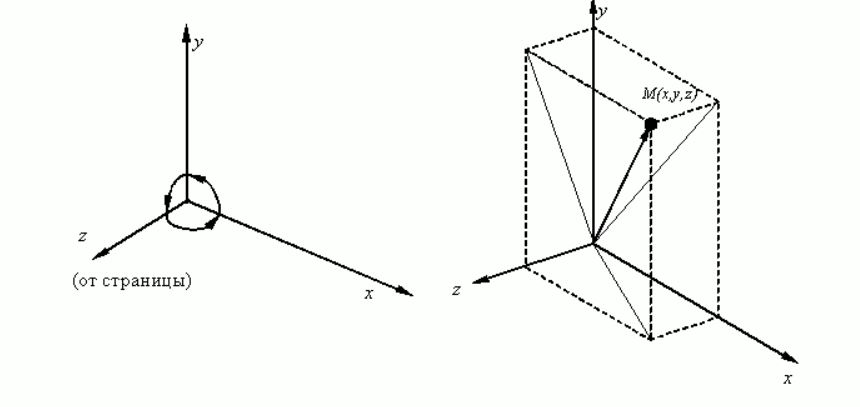
\includegraphics[scale=1]{source/3dCoords.jpg}}
		\caption{Алгоритм отрисовки траекторий}
	\end{figure}		
	
	
	
	 Для реализации трехмерных преобразований с помощью матриц необходимо перейти к однородным координатам (x,y,z,1).
	
	Тогда матрица трехмерного преобразования  (переноса, масштабирования, поворота) в общем виде будет следующей:
	
	$$
	A = 
	\begin{pmatrix} 
		a_{11} & a_{12} & a_{13} & a_{14} \\
		a_{21} & a_{22} & a_{23} & a_{24} \\
		a_{31} & a_{32} & a_{33} & a_{34} \\
		a_{41} & a_{42} & a_{43} & a_{44} \\
		\end{pmatrix},
	A_1 = 
	\begin{pmatrix} 
		a_{11} & a_{12} & a_{13} \\
		a_{21} & a_{22} & a_{23} \\
		a_{31} & a_{32} & a_{33} \\
		a_{41} & a_{42} & a_{43} \\
	\end{pmatrix},
	\quad
	$$
	
	где матрица $A_1$ осуществляет линейное преобразование в виде изменения масштаба, сдвига и вращения,
	вектор $(a_{41},a_{42},a_{43})$ производит перенос объекта, а вектор-столбец $(a_{14},a_{24},a_{34})^T$ -
	преобразования в перспективе. Скалярный элемент $a_{44}$ выполняет общее изменение масштаба.
	
	\subsubsection{Матрица трехмерного переноса}
	$$
	T(D_x, D_y, D_z) = 
	\begin{bmatrix} 
		1 & 0 & 0 & 0 \\
		0 & 1 & 0 & 0 \\
		0 & 0 & 1 & 0 \\
		D_x & D_y & D_z & 1 \\
	\end{bmatrix},
	\quad
	$$
	при этом
	
	\begin{equation}
		[x, y, z, 1] \cdot T(D_x, D_y, D_z) =[x + D_x, y + D_z, z + D_z, 1]
	\end{equation}
		
	\subsubsection{Операция масштабирования}
	$$
	S(S_x, S_y, S_z) = 
	\begin{bmatrix} 
		S_x & 0 & 0 & 0 \\
		0 & S_y & 0 & 0 \\
		0 & 0 & S_z & 0 \\
		0 & 0 & 0 & 1 \\
	\end{bmatrix},
	\quad
	$$
	при этом
	
	\begin{equation}
		[x, y, z, 1] \cdot S(S_x, S_y, S_z) = [S_x \cdot x, S_y \cdot y, S_z \cdot z, 1]
	\end{equation}	
	
	
	\subsubsection{Трехмерный сдвиг}
	\begin{equation}
		[x, y, z, 1] \cdot 
		\begin{bmatrix} 
			1 & b & c & 0 \\
			d & 1 & f & 0 \\
			h & i & 1 & 0 \\
			0 & 0 & 0 & 1 \\
		\end{bmatrix} = [x + yd + hz, bx + y + iz, cx + fy + z, 1].
		\quad
	\end{equation}	
			
	\subsubsection{Трехмерное вращение}
	В трехмерном пространстве поворот вокруг оси Z описывается матрицей
	$$
	R_z(a) = 
	\begin{bmatrix} 
		cos(a) & sin(a) & 0 & 0 \\
		-sin(a) & cos(a) & 0 & 0 \\
		0 & 0 & 1 & 0 \\
		0 & 0 & 0 & 1 \\
	\end{bmatrix},
	\quad
	$$

	Матрица поворота вокруг оси X имеет вид
	$$
	R_x(a) = 
	\begin{bmatrix} 
		1 & 0 & 0 & 0 \\
		0 & cos(a) & sin(a) & 0 \\
		0 & -sin(a) & cos(a) & 0 \\
		0 & 0 & 0 & 1 \\
	\end{bmatrix},
	\quad
	$$
	
	и вокруг оси Oy:
	$$
	R_y(a) = 
	\begin{bmatrix} 
		cos(a) & 0 & -sin(a) & 0 \\
		0 & 1 & 0 & 0 \\
		sin(a) & 0 & cos(a) & 0 \\
		0 & 0 & 0 & 1 \\
	\end{bmatrix},
	\quad
	$$
		
		
	\subsection{Алгоритм построения Земли}
	Для начала нужно записать в массив точки для построения широт и меридианов модели Земли. Алгоритм данных действий представлен ниже\newline на Рисунке 2.
	%\par $geo\_to\_rect$ - функция для перевода координат из геодезической системы координат в прямоугольную.
	
	\clearpage
	\begin{figure}[h!]
		\centering{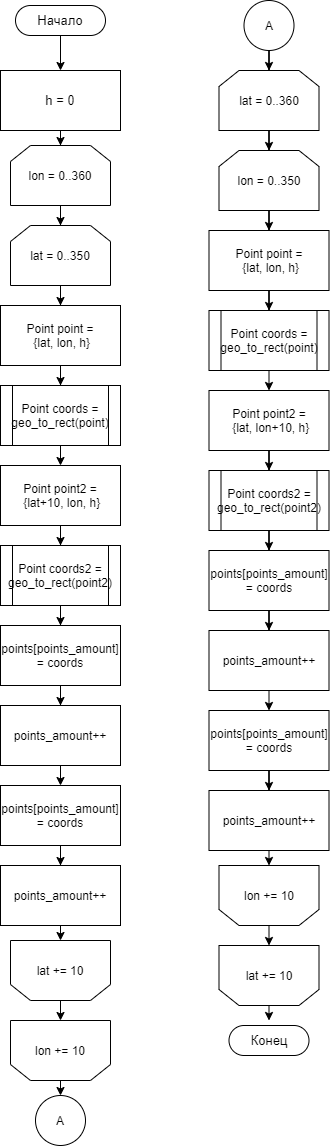
\includegraphics[scale=0.6]{source/init_earth.png}}
		\caption{Алгоритм записи точек для широт и меридианов модели Земли }
	\end{figure}
	\clearpage
	
	
	Затем следует использовать следующий алгоритм для отрисовки полученных точек прямоугольной системы
	координат. Схема алгоритма изображена ниже на Рисунке 3.
	
	\begin{figure}[h!]
		\centering{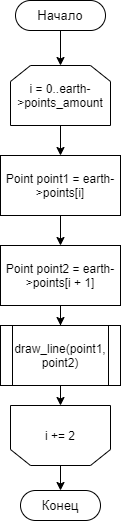
\includegraphics[scale=0.9]{source/draw_earth.png}}
		\caption{Алгоритм для отрисовки полученных точек}
	\end{figure}		
	Последний алгоритм вызывается каждый раз при изменении положения модели Земли.	
	\clearpage	
	
	
	\subsection{Алгоритм построения траекторий}
	После построения модели Земли можно отображать траектории перемещения воздушных судов. Алгоритм показан ниже на Рисунке 4.
	 
	 \begin{figure}[h!]
	 	\centering{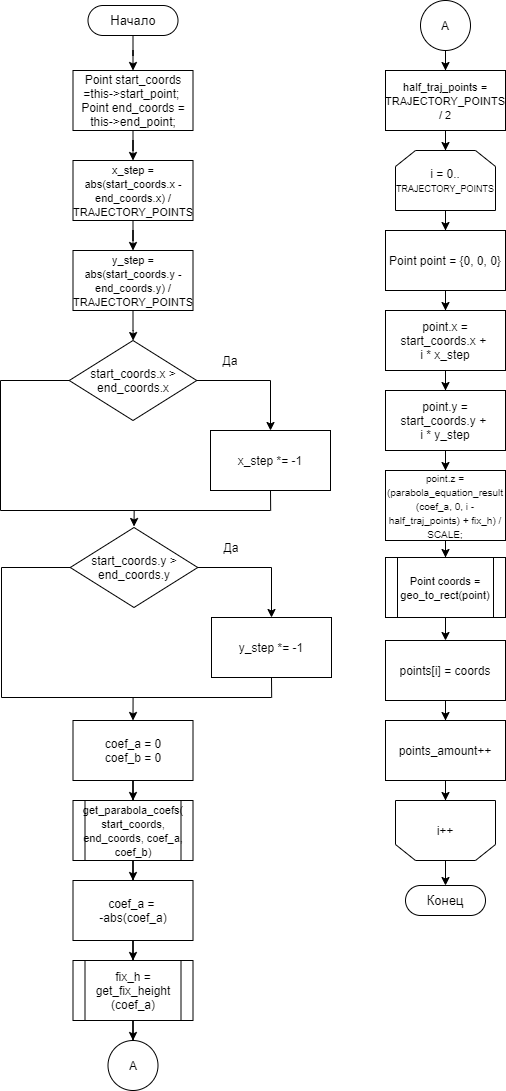
\includegraphics[scale=0.55]{source/build.png}}
	 	\caption{Алгоритм генерации и записи точек траектории}
	 \end{figure}		
	 \clearpage
	
	Затем следует использовать следующий алгоритм для отрисовки полученных точек траектории прямоугольной системы координат. Схема алгоритма изображена ниже на Рисунке 5.
	
	\begin{figure}[h!]
		\centering{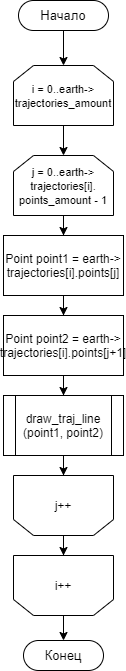
\includegraphics[scale=0.8]{source/draw_trajectories.png}}
		\caption{Алгоритм отрисовки траекторий}
	\end{figure}		
	\clearpage
	
	
	\subsection{Используемые типы и структуры данных}
	Необходимо реализовать следующие типы и структуры данных:
	\begin{itemize}
		\item[1)] "земля" - хранит точки текущего положения планеты и массив траекторий движения;
		\item[2)] траектория - хранит точки траектории движения самолета;
		\item[3)] список траекторий;
		\item[4)] сцена - хранит в себе описанные выше структуры;
		\item[5)] точка - хранит координаты x, y, z;
		\item[6)] интерфейс - использует библиотечные классы для предоставления доступа к интерфейсу.
		
	\end{itemize}
	
	\subsection*{Вывод}
	\addcontentsline{toc}{subsection}{Вывод}
	Таким образом, в данном разделе были представлены требования к программе, алгоритм решения поставленной задачи, а именно построение модели земли и траекторий. Представлены схемы алгоритмов решения этих подзадач. Также были представлены используемые типы и структуры данных.
 	\newpage
	
	\section{Технологический раздел}
	В данном разделе будут рассмотрены средства реализации, сведения о модулях
	программы, её структуры и состав классов, интерфейс.

	\subsection{Средства реализации}
	В качестве языка программирования был выбран C++, так как:
	
	\begin{itemize}
		\item[1)] я знаком с данным языком программирования, имею представление о
		способах тестирования программы;
		\item[2)] данный язык программирования объектно-ориентирован.		
	\end{itemize}
	
	В качестве среды разработки была выбрана "Qt" так как:
	\begin{itemize}
		\item[1)] я знаком с данной средой разработки;
		\item[2)] она является бесплатной;
		\item[3)] с минимальными изменениями написанный код	может быть исполнен как на Windows,
		 так и на Linux. 	
	\end{itemize}
	\newpage
	
	\subsection{Реализация без OpenGL}
	Описание программы, реализованной без библиотеки OpenGL.
	\subsubsection{Сведения о модулях программы}
	В состав программы входят:
	\begin{itemize}
		\item[1)] main.c - главный файл программы, в котором располагается точка входа в программу;
		\item[2)] mainwindow.ui - интерфейс программы;
		\item[3)] mainwindow.c - реализация интерфейса;
		\item[4)] maincwindow.h - header файл mainwindow.c;
		\item[5)] earth.c - "земля";
		\item[6)] earth.h - header файл earth.c;
		\item[7)] points.c - структура "точка" и функции, связанные с ней;
		\item[8)] point.h - header файл point.c;
		\item[9)] trajectory.c - траектория;
		\item[10)] trajectory.h - header файл trajectory.c;
		\item[11)] consts.h - константы.	 	
	\end{itemize}

	\newpage
	\subsubsection{Структура и состав классов}
	Программа содержит классы и структуру, изображенные на Рисунке 6:
	\begin{figure}[h!]
		\centering{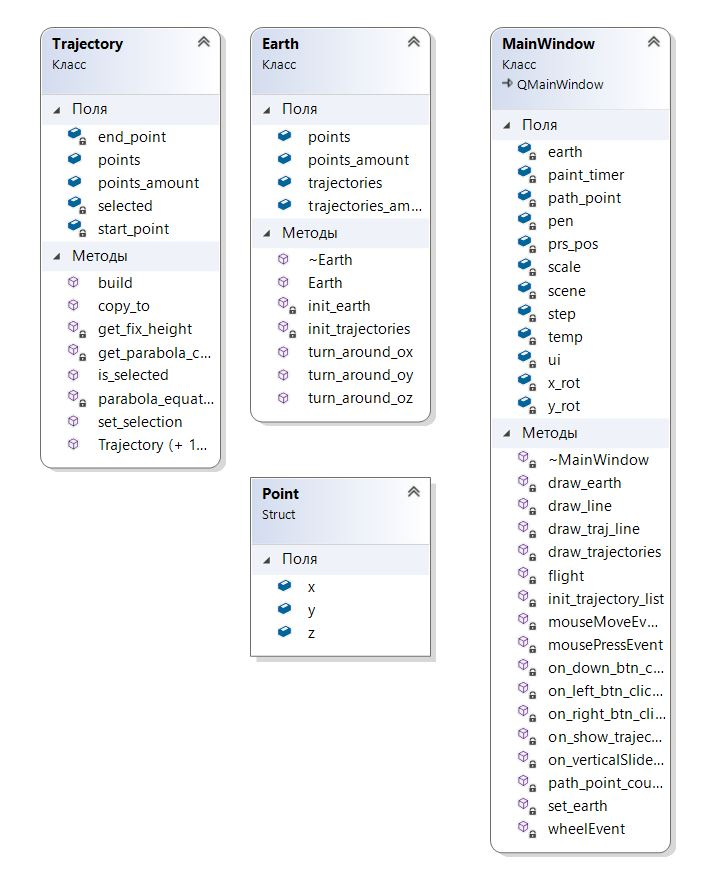
\includegraphics[scale=1]{source/structure.jpg}}
		\caption{Структура и состав классов}
	\end{figure}	
	\clearpage
	
	\subsection{Реализация c OpenGL}
	Описание программы, реализованной c библиотекой OpenGL.
	
	\subsubsection{Сведения о модулях программы}
	В состав программы входят:
	\begin{itemize}
		\item[1)] main.c - главный файл программы, в котором располагается точка входа в программу;
		\item[2)] mainwindow.ui - интерфейс программы;
		\item[3)] mainwindow.c - реализация интерфейса;
		\item[4)] maincwindow.h - header файл mainwindow.c;
		\item[5)] earthogl.c - "земля" и отображающая сцена;
		\item[6)] earthogl.h - header файл earth.c;
		\item[7)] points.c - структура "точка" и функции, связанные с ней;
		\item[8)] point.h - header файл point.c;
		\item[9)] trajectory.c - траектория;
		\item[10)] trajectory.h - header файл trajectory.c;
		\item[11)] consts.h - константы.		 	
	\end{itemize}
	
	\newpage
	\subsubsection{Структура и состав классов}
	Программа содержит классы и структуру, изображенные на Рисунке 7:
	\begin{figure}[h!]
		\centering{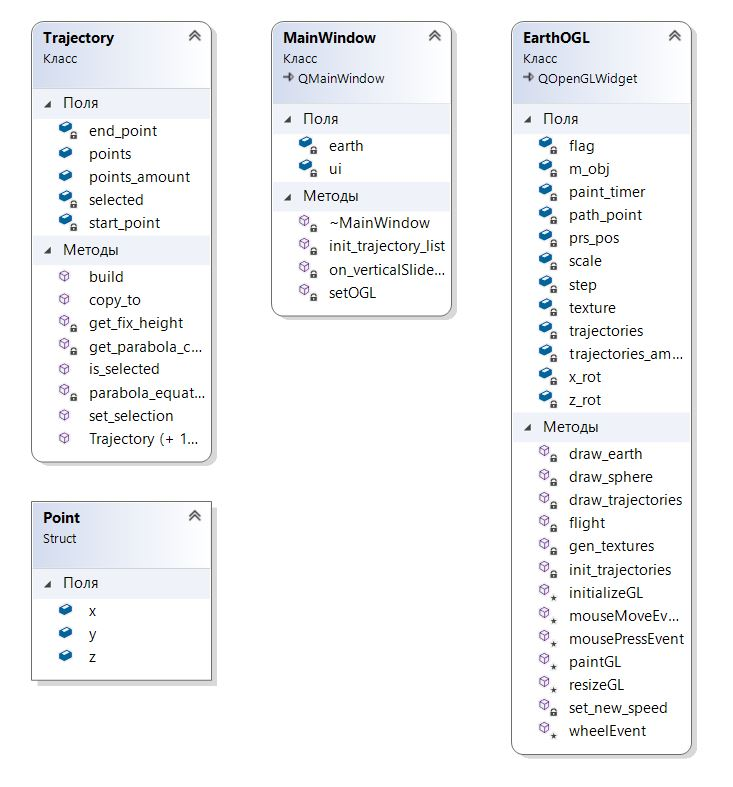
\includegraphics[scale=1]{source/structureOGL.jpg}}
		\caption{Алгоритм генерации и записи точек траектории}
	\end{figure}	
	\clearpage

	\subsection{Интерфейс программы}
	Слева расположен список доступных для отображения траекторий.\par
	Ниже находится слайдер для регулировании скорости передвижения самолетов.\par
	Справа показана интерактивная сцена со всей визуальной составляющей программы.
	
	\begin{figure}[h!]
		\centering{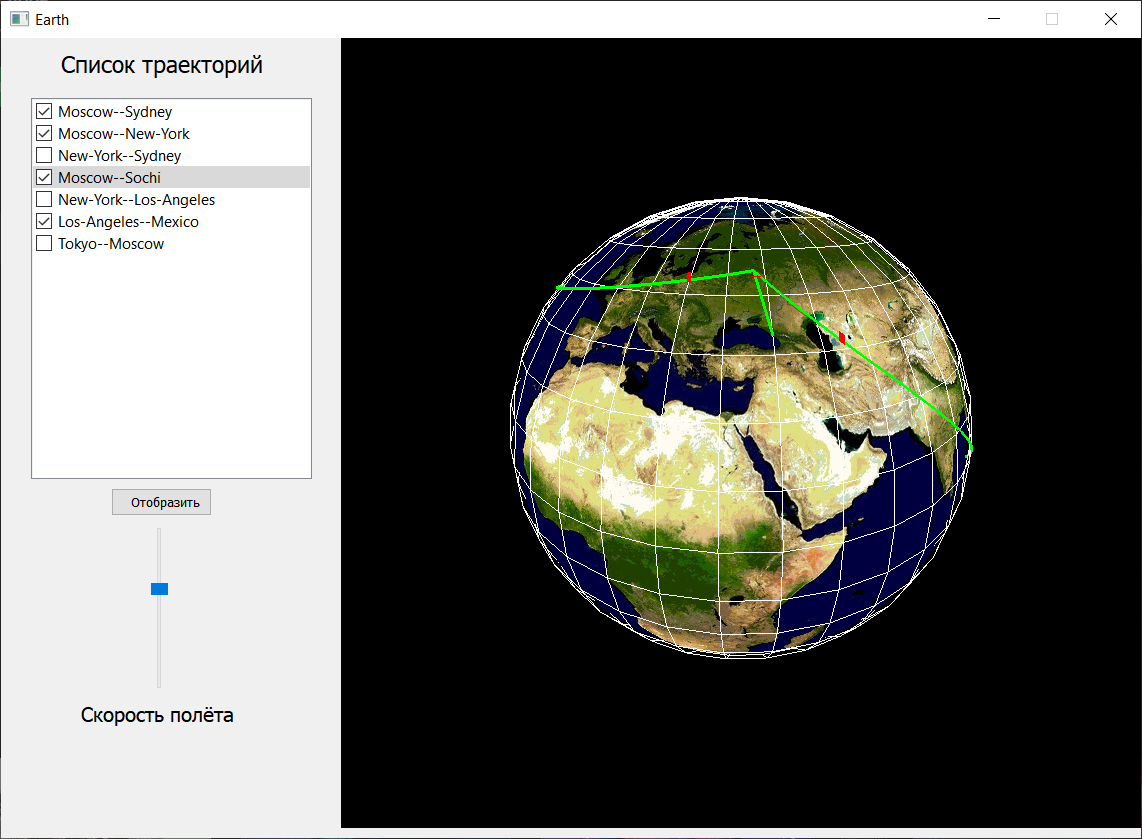
\includegraphics[scale=0.7]{source/interface.png}}
		\caption{Интерфейс программы}
	\end{figure}	

	\subsection*{Вывод}
	\addcontentsline{toc}{subsection}{Вывод}
	В данном разделе были представлены средства реализации, сведения о
	модулях программы, структура и состав классов и интерфейс программы.
	
	\newpage
	\section{Экспериментальный раздел}
	В данном разделе будут представлены примеры работы программы и
	проведены эксперименты.
	
	\subsection{Описание экспериментов}
	В серии экспериментов получится узнать, какая вариация программы (без использования библиотеки OpenGL и с её использованием) работает быстрее и на сколько.\par
	Для замеров процессорного времени используется класс Qt $QTime$.\par
	Ниже на Рисунке 9 для каждой версии представлена зависимость времени от кол-ва поворотов модели.\par  
	\begin{figure}[h!]
		\begin{tikzpicture}
			
			\begin{axis}[
				axis lines = left,
				xlabel = Кол-во поворотов,
				ylabel = {Время, мсек},
				legend pos=north west,
				ymajorgrids=true,
				xmajorgrids=true,
				width = 400
				]
				\addplot[color=red, mark=*] table[x index=0, y index=1] {pr.dat}; 
				\addplot[color=blue, mark=*] table[x index=0, y index=1] {prOGL.dat};
				
				\addlegendentry{Без OpenGl}
				\addlegendentry{C OpenGL}
				
			\end{axis}
		\end{tikzpicture}
		\caption{График зависимости времени от кол-ва поворотов модели}
	\end{figure}
	  
	Видно, что использование библиотеки OpenGL повышает скорость преобразований в больше чем 1500 раз в сравнение с моей реализацией. Так же можно сделать очевидный вывод, что при увеличении количества операций увеличивается и затрачиваемое время.
	

	\subsection{Примеры работы программы}
	Ниже на Рисунке 10 и Рисунке 11 будут представлены примеры работы программы.
	
	\begin{figure}[h!]
		\centering{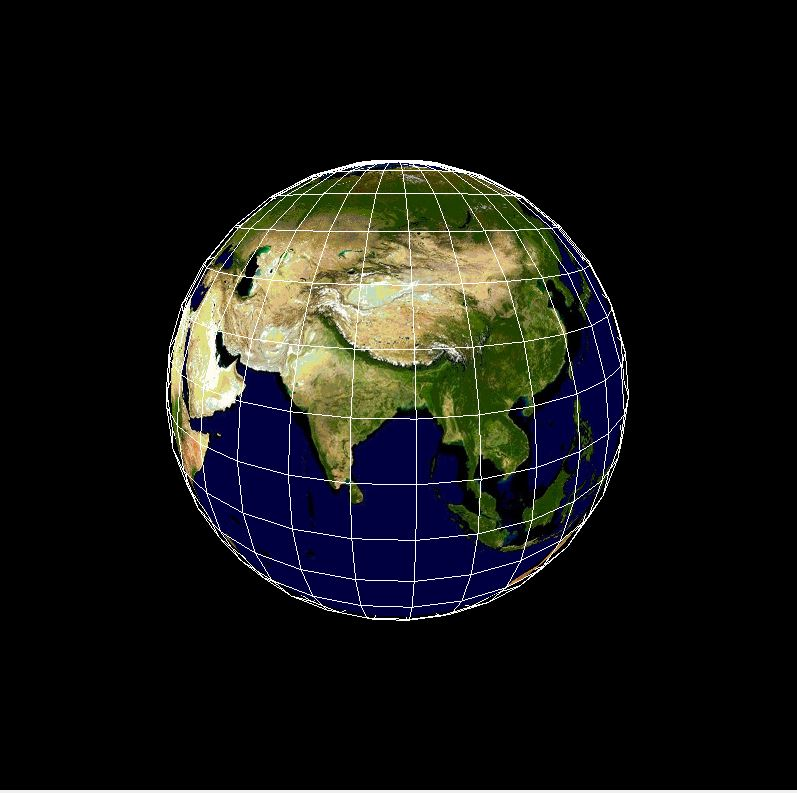
\includegraphics[scale=0.8]{source/emptyScene.jpg}}
		\caption{Начальная сцена}
	\end{figure}
	\newpage
	
	\begin{figure}[h!]
		\centering{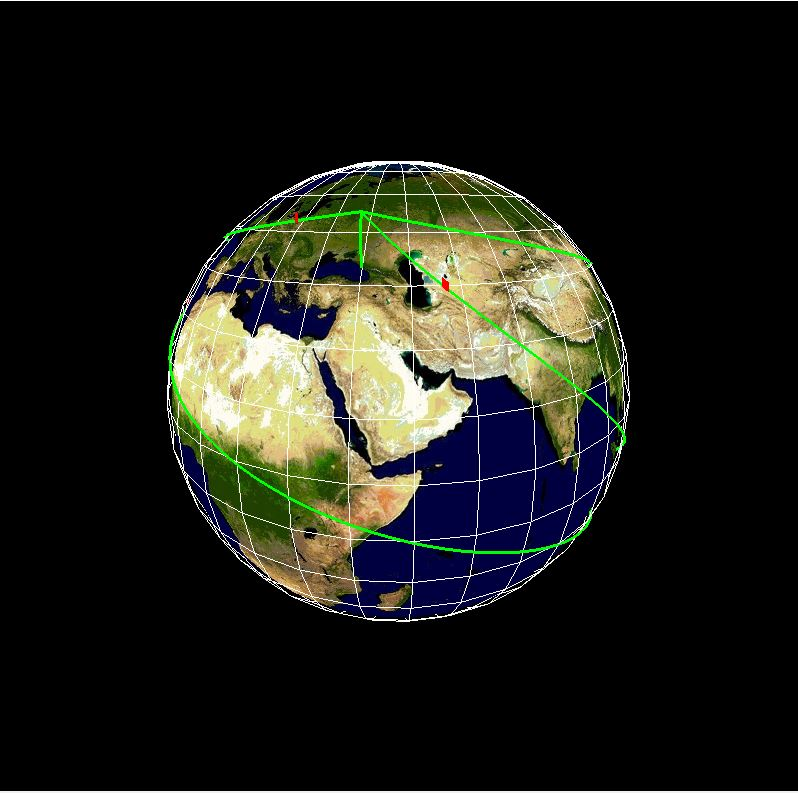
\includegraphics[scale=0.8]{source/fullScene.jpg}}
		\caption{Заполненная сцена}
	\end{figure}
	
	Белым цветом показаны мередианы и широты.\par
	Зелёным изображены траектории передвижений самолетов.\par
	Красным - сами передвигающиеся самолёты.\par

	\subsection*{Вывод}
	\addcontentsline{toc}{subsection}{Вывод}
	В данном разделе были представлены примеры работы программы и
	проведены эксперименты, в ходе которых выяснилось, что использование библиотеки OpenGL сильно повышает скорость
	работы программы.
	
	\newpage
	\section*{Заключение}
	\addcontentsline{toc}{subsection}{Заключение}
	В данной работе была создана трёхмерная модель Земли с визуализацией полётов самолетов с различными возможностями:
	
	\begin{itemize}
		\item[1)] поворот модели в любом направлении;
		\item[2)] масштабирование модели;
		\item[3)] список доступных для выбора траекторий;
		\item[4)] отображение траектории полетов;
		\item[5)] отображение передвижений самолетов по данным траекториям.
		
	\end{itemize}\par
	
	Была разработана версия программы использующая библиотеку OpenGL.
	
	Также были проведены эксперименты, в результате которых было выявлено, что использование OpenGL позволяет ускорить преобразования модели, и тем самым улучшить визуальный опыт использования программы пользователем.

	\clearpage	
	\section*{Литература}
	\addcontentsline{toc}{section}{Литература}
		
	\begin{enumerate}
		\label{CPlusPlus}
		\item[1)] Бьерн Страуструп. Язык программирования С++. -URL:\par 
		\href{https://codernet.ru/books/c_plus/bern_straustrup_yazyk_programmirovaniya_c_specialnoe_izdanie/}
		{https://codernet.ru/books/c\_plus/bern\_straustrup\_yazyk\_programmirovaniya\_
			c\_specialnoe\_izdanie/}\par(дата обращения:
		01.10.2020). Текст: электронный.
		
		\label{Cute}
		\item[2)] Qt. -URL:\par
		\href{https://www.qt.io/}{https://www.qt.io/} (дата обращения: 01.10.2020). Текст: электронный.
		
		\item[3)] Трехмерные преобразования и проекции. -URL:\par
		\href{http://compgraph.tpu.ru/3d.htm}{http://compgraph.tpu.ru/3d.htm} (дата обращения: 23.12.2020). Текст: электронный.
		
		\item[4)] Трехмерные матричные преобразования. -URL:\par
		\href{http://www.astro.tsu.ru/KGaG/text/5_2.html}{http://www.astro.tsu.ru/KGaG/text/5\_2.html} (дата обращения: 23.12.2020). Текст: электронный.
		
		\item[5)] Траектория. -URL:\par
		\href{http://av-physics.narod.ru/mechanics/trajectory.htm}{http://av-physics.narod.ru/mechanics/trajectory.htm} (дата обращения: 23.12.2020). Текст: электронный.
		
		\item[6)] Мировая гражданская авиация сегодня. -URL:\par
		\href{https://promvesti.com/mirovaya-grazhdanskaya-aviaciya-segodnya/}{https://promvesti.com/mirovaya-grazhdanskaya-aviaciya-segodnya/} (дата обращения: 23.12.2020). Текст: электронный.
		
		\item[7)] Планета Земля краткое описание. -URL:\par
		\href{https://cosmosplanet.ru/solnechnayasistema/zemlya/zemlya-opisanie.html}{https://cosmosplanet.ru/solnechnayasistema/zemlya/zemlya-opisanie.html} (дата обращения: 23.12.2020). Текст: электронный.
		
		\newpage
		\item[8)] Аффинные преобразования. -URL:\par
		\href{https://ru.wikibooks.org/wiki/Аффинные_преобразования}{https://ru.wikibooks.org/wiki/Аффинные\_преобразования} (дата обращения: 23.12.2020). Текст: электронный		
		
		\item[9)] Преобразования геодезических систем координат. -URL:\par
		\href{https://studref.com/}{https://studref.com/} (дата обращения: 23.12.2020). Текст: электронный.
		
		\item[10)] Географические координаты городов. -URL:\par
		\href{https://dateandtime.info/ru/citycoordinates.php?id=3451190}{https://dateandtime.info/ru/citycoordinates.php?id=3451190} (дата обращения: 23.12.2020). Текст: электронный.
		
		\item[11)] Аффинные преобразования. -URL:\par
		\href{https://gsg.mskobr.ru/files/Proekt/himiya1.pdf}{https://gsg.mskobr.ru/files/Proekt/himiya1.pdf} (дата обращения: 23.12.2020). Текст: электронный.
		
		
	\end{enumerate}
\end{document}